\lstset{language=Ruby}
\newpage

\section{Seitenaufbau in LaTeX}
Der Seitenaufbau wird vollständing in der Präambel definiert, von der Seitengröße über die Abstände der Seitenränder bishin zu den Zitationsstilen sowie dem Inhaltsverzeichnis. Das macht den Umgang mit \LaTeX{} für eine wissenschaftliche Arbeit so attraktiv. Grundsätzlich erlaubt es der Workflow von \LaTeX{}, sich vollständig auf den Inhalt zu konzentrieren und so wenig wie nötig sich mit \glqq Design\grqq\ aufzuhalten.


Dieses Dokument nutzt die Dokumentenklasse scrreprt\footcite[S. 51]{kohmKOMA2019} aus dem Paket KOMA-Script. Diese hat sich für unseren Einsatzzweck bereits vielfach bewährt und sollte somit ein sicheres Mittel sein. Die Dokumentenklasse gibt an, um was für ein Dokument es sich handelt\footcite[vgl. ][S. 9]{oetikerIntroductionLATEX2e2018}.

\section{Funktionen von LaTeX}

\subsection{Textformatierung}
Da dies hier den Rahmen sprengen würde, möchte ich auf eine sehr gute, kostenfreie Einführung verweisen, welche Kompakt und gut verständlich die Feinheiten von \LaTeX{} erklärt. Über sechs Kapitel wird dann angefangen bei der grundsätzlichen Struktur eines Dokumentes bis hin dazu, wie man Grundlegende Funktionen von \LaTeX{} umschreibt\footcite{oetikerIntroductionLATEX2e2018}, und das alles auf 153 Seiten, kostenlos.

\subsection{Mathematische Schreibumgebung}
Wenn man Code zwischen zwei Dollar Zeichen \$ \dots\ \$ schreibt, schreibt man in dem mathematischen Modus. Alles darin wird interpretiert und durch entsprechende Symbole ersetzt. Das Ergebnis spricht für sich.

1)

$ SEW\footnote{Summe der Endwerte} (RF\footnote{Rückflüsse}) = \sum_{t=1}^{n} [ ( E_{t} - A_{t}) \times (1+i)\ ^{N-t}] $

$ SEW(RF) = 5\times1,1^{5}+10\times1,1^{4}+15\times1,1^{3}+10\times1,1^{2}+30\times1,1^{1}+35 = 122,76$


$ i_{m} = \sqrt[N]{\dfrac{SEW(RF)}{BW(IA)}} -1$

$ i_{m} = \sqrt[6]{\dfrac{122,76}{50}} -1 = 0,1615 \approx 16,15\%$

2)

$ SEW(RF) = 186,72 $

$ i_{m} = 0,1097 \approx 10,97\%$
\begin{lstlisting}
1)

$ SEW\footnote{Summe der Endwerte} (RF\footnote{Rückflüsse}) = \sum_{t=1}^{n} [ ( E_{t} - A_{t}) \times (1+i)\ ^{N-t}] $

$ SEW(RF) = 5\times1,1^{5}+10\times1,1^{4}+15\times1,1^{3}+10\times1,1^{2}+30\times1,1^{1}+35 = 122,76$


$ i_{m} = \sqrt[N]{\dfrac{SEW(RF)}{BW(IA)}} -1$

$ i_{m} = \sqrt[6]{\dfrac{122,76}{50}} -1 = 0,1615 \approx 16,15\%$

2)

$ SEW(RF) = 186,72 $

$ i_{m} = 0,1097 \approx 10,97\%$
\end{lstlisting}

Grundsätzlich unterstützt \LaTeX{} aber noch eine weitere Methode, mathematische Sequenzen darzustellen.

\[
  \varphi = \frac{1 + \sqrt{5}}{2} = 1.618 \ldots
\]

\begin{lstlisting}
\[
  \varphi = \frac{1 + \sqrt{5}}{2} = 1.618 \ldots
\]
\end{lstlisting}
Man unterscheidet beide Methoden in 1) \emph{Inline math} und 2) \emph{Displayed math}\footcite[Vgl. ][S.276]{kottwitzLaTeXCookbook902015}. Inline math eignet sich, um Formeln im Text einzufügen, Displayed math präsentiert die Formel in einer eigenen Zeile.
%Eine sehr gute Übersicht findet man kostenfrei von Michael Doobs\footcite[S. 33ff]{michaeldoobGentleIntroductionTEX}.

\subsection{Fußnoten}
Fußnoten werden über den Befehl \textbackslash footnote gesetzt und automatisch im Footer fortlaufend Nummeriert aufgeführt.\footnote{\href{https://de.wikibooks.org/wiki/LaTeX-W\%C3\%B6rterbuch:_footnote}{Mehr auf Wikibooks}}
\begin{lstlisting}
Fußnoten werden über den Befehl \footnote{Meine erste Fußnote} gesetzt und automatisch im Footer fortlaufend Nummeriert aufgeführt.\footnote{\href{https://de.wikibooks.org/wiki/LaTeX-W\%C3\%B6rterbuch:_footnote}{Mehr auf Wikibooks}}
\end{lstlisting}

\subsection{Querverweise}

\subsection{Code}
Code wird wie folgt eingefügt
\begin{lstlisting}
#!/usr/bin/env ruby

listofstrings = ARGV
puts listofstrings.sort.uniq

\end{lstlisting}
Sollte man diese Funktion nicht gebrauchen, kann man die letzten Zeilen in der Präambel deaktivieren, damit die Pakete nicht zwingend geladen werden müssen.
\subsection{Quellcode zitieren}

\subsection{Tabellen}
\begin{table}[htbp]
\begin{tabular}{|l|l|l|l|l|l|l|}
\hline
t & 0 & 1 & 2 & 3 & 4 & 5 \\ \hline
lfd. EZÜ & 262.500 & 352.450 & 455.395 & 572.871 & 706.628 & 858.656 \\ \hline
zstl. ZÜ &  & 89.950 & 192.895 & 310.371 & 444.128 & 596.156 \\ \hline
Barwerte & -550.000 & 84.065 & 168.482 & 253.355 & 338.823 & 425.051 \\ \hline
kumulierter Barwert & 719.776 &  &  &  &  &  \\ \hline
\end{tabular}
\caption{Eine einfache Tabelle}
\end{table}

\begin{lstlisting}
\begin{table}[htbp]
\begin{tabular}{|l|l|l|l|l|l|l|}
\hline
t & 0 & 1 & 2 & 3 & 4 & 5 \\ \hline
lfd. EZÜ & 262.500 & 352.450 & 455.395 & 572.871 & 706.628 & 858.656 \\ \hline
zstl. ZÜ &  & 89.950 & 192.895 & 310.371 & 444.128 & 596.156 \\ \hline
Barwerte & -550.000 & 84.065 & 168.482 & 253.355 & 338.823 & 425.051 \\ \hline
kumulierter Barwert & 719.776 &  &  &  &  &  \\ \hline
\end{tabular}
\caption{Eine einfache Tabelle}
\end{table}
\end{lstlisting}

Ein Tipp zum Thema Tabellen: nutzt ein externes Tool. Viele Editoren bringen Tools mit, um Tabellen einfacher zu erstellen. Ich finde folgende Webseite sehr Hilfreich \href{https://tablesgenerator.com}{https://tablesgenerator.com}.

\subsection{Grafiken}
Grafiken werden von LaTeX dahin gesetzt, wo sie am besten hinpassen.

\begin{figure}[htbp]
  \centering
     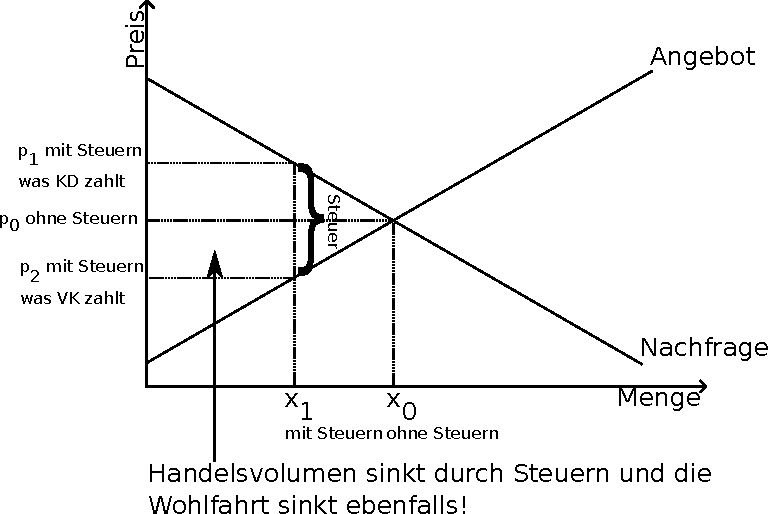
\includegraphics[]{ProdKonsRentemitSteuern.pdf}
  \caption{Die Besteuerung eines Marktes}
  \label{fig:Bild1}
\end{figure}

\begin{lstlisting}
\begin{figure}[htbp]
  \centering
     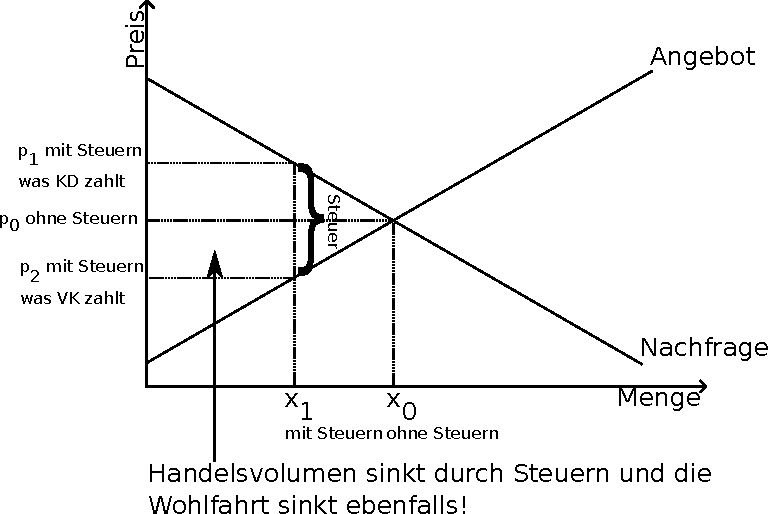
\includegraphics[]{ProdKonsRentemitSteuern.pdf}
  \caption{Die Besteuerung eines Marktes}
  \label{fig:Bild1}
\end{figure}
\end{lstlisting}

Abbildung Zwei zeigt eine Grafik, die zu groß für diese Seite wäre. LaTeX meldet das über eine Warnung im log. Auch dieses Thema findet man ausreichend über das Internet erklärt. In unserem Fall reicht es, die Größe des Bildes anzupassen. Das geschieht mit einem zusätzlichem Parameter

\begin{figure}[htbp]
  \centering
     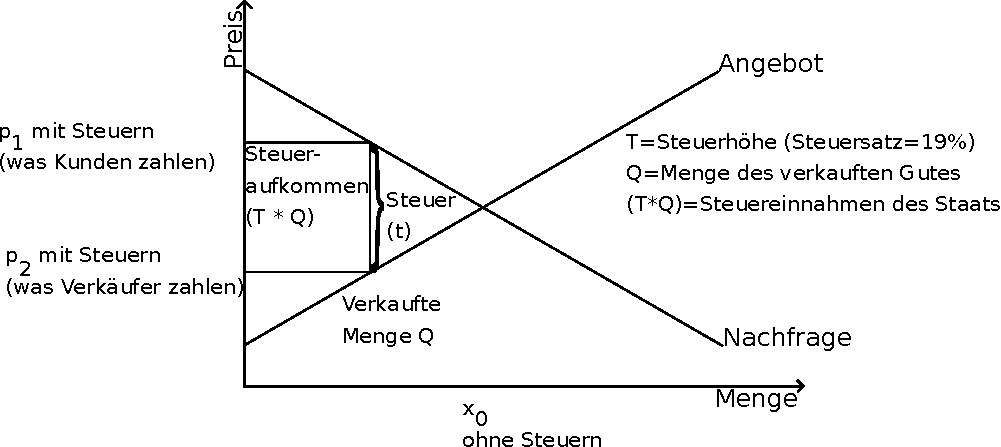
\includegraphics[width=1\linewidth]{PMSteuer.pdf}
  \caption{Steueraufkommen}
  \label{fig:Bild2}
\end{figure}

\begin{lstlisting}
\begin{figure}[htbp]
  \centering
     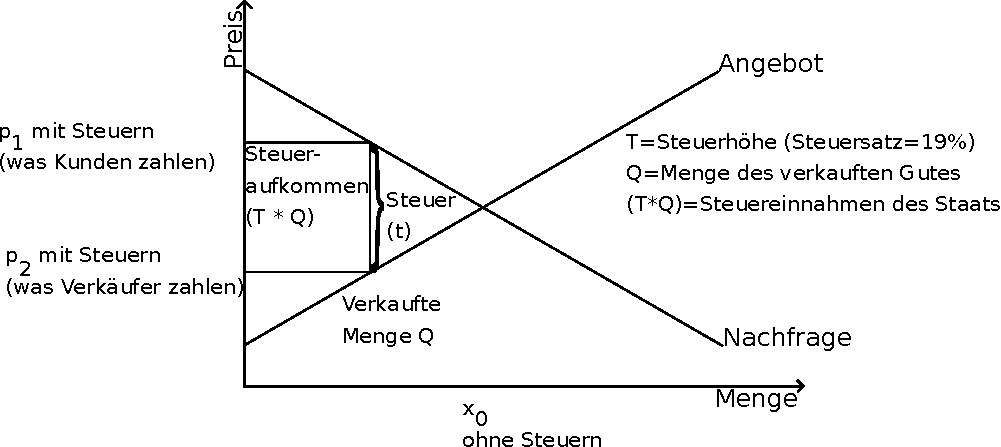
\includegraphics[width=1\linewidth]{PMSteuer.pdf}
  \caption{Steueraufkommen}
  \label{fig:Bild2}
\end{figure}
\end{lstlisting}
\subsection{Zitieren}
Es scheint, als würde jeder Professor seine persönlichen Vorlieben zum verwendeten Zitationsstil haben. Hier sollen also verschiedene Stile ausprobiert werden, so dass man nicht viel Zeit damit verliert.

Dieses Buch wurde mit Hilfe der üblichen Internetadressen (vorwiegend \href{https://tex.stackexchange.com/}{TeX - LaTeX Stack Exchange} ) aber auch dem Buch \glqq Wissenschaftliche Arbeiten schreiben mit LaTeX\grqq{} von Joachim Schlosser\footcite{schlosserWissenschaftlicheArbeitenSchreiben2014} geschrieben.
\subsection{Verzeichnisse}
\LaTeX{} macht es verhältnismäßig einfach, Verzeichnisse zu führen. Anbei sind folgende hier im Code verwendete erklärt.
\subsection{Abkürzungsverzeichnis}
Here is some text, where we use APC.\nomenclature{APC}{antigeen-presenterende cel}
\subsubsection{Glossar}
Ein Glossar soll dem Leser Fachbegriffe näher bringen. In einem gesonderten Verzeichnis im Anhang werden die definierten Begriffe dann aufgelistet.

Der Code ist meta/gls.tex definiert.
\subsubsection{Index}
Schreiben sie von \index{Alpha}Alpha bis \index{Omega}Omega.
\begin{lstlisting}
Schreiben sie von \index{Alpha}Alpha bis \index{Omega}Omega.
\end{lstlisting}

Mit einem Index kann man Schlagworte und Themengruppen zusammenfassen und dem Leser helfen, diese im Dokument zu finden.
